\documentclass[12pt]{article}
\usepackage{amsmath}
\usepackage{multirow}
\usepackage{enumerate}
\usepackage{graphicx}
\usepackage{changepage}
\usepackage{textcomp}

\setlength{\voffset}{-3cm}
\setlength{\hoffset}{-2cm}
\setlength{\parindent}{0cm}
\setlength{\textheight}{27cm}
\setlength{\textwidth}{17cm}


\begin{document}

\quad\\[2cm]

\begin{center}
{\Huge Statistics for Computing MA4413\\[0.8cm]
Midterm Examination 1\\[1cm]
{\bf Type B}}\\[2cm]
\end{center}

\begin{itemize}\itemsep0.6cm
\item Do not turn over the page until instructed to do so.
\item Rough work pages are provided within.
\item Useful formulae and Binomial tables are provided at the back.
\item {\bf Enter your answers (using an ``X'') in the table on the last page.}
\item There are 15 questions in total.
$
\text{Each question answered } \left\{\begin{array}{rr}
\text{correctly } = & \hspace{-0.2cm}1\%. \\[0.2cm]
\text{incorrectly } = & \hspace{-0.2cm}-\tfrac{1}{3}\%.
\end{array}\right.
$
%(\emph{there are no negative marks}).
\item For each question, only \emph{one} answer is correct.
\item Scientific calculators approved by the University of Limerick can be used.
\end{itemize}

\newpage
\section*{Questions 1 - 5}

\rule{\linewidth}{1pt}
\quad\\
{\bf Q1} The time it takes you to complete this exam is an example of which type of data?\\[0.2cm]
\begin{tabular}{cccc}
{\bf(a)} numeric discrete & {\bf(b)} categorical  & {\bf(c)} numeric continuous & {\bf(d)} infinite\\[0.6cm]
\end{tabular}


\rule{\linewidth}{1pt}
\quad

A large online retailer believes that its customers spend on average {\sffamily\texteuro}55 per transaction. Each week over 100,000 transactions are made. Thus, a random sample of 500 transactions were selected and the sample average was found to be {\sffamily\texteuro}63.20.\\[0.3cm]

{\bf Q2} What is the parameter here?\\[0.2cm]
\begin{tabular}{cccc}
{\bf(a)} $\mu =$ unknown & {\bf(b)} $n = 100,000$ & {\bf(c)} $p =$ unknown & {\bf(d)} $\mu = 55$ \\[0.6cm]
\end{tabular}

{\bf Q3} What is the statistic here?\\[0.2cm]
\begin{tabular}{cccc}
{\bf(a)} $\hat p = \frac{63.20}{500}$ & {\bf(b)} $\hat p = \frac{500}{100,000}$ & {\bf(c)} $\mu = 55$ & {\bf(d)} $\bar x = 63.20$ \\[0.6cm]
\end{tabular}



\rule{\linewidth}{1pt}

\quad\\
Consider the following sample of ages of mechanical components:
\begin{center}
\begin{tabular}{|cccccc|}
\hline
&&&&&\\[-0.4cm]
3 & 5 & 4 & 12 & 4 & 8\\
\hline
\multicolumn{6}{c}{}
\end{tabular}
\end{center}


{\bf Q4} What is the value of the sample variance?\\[0.2cm]
\begin{tabular}{cccc}
{\bf(a)} $11.6$ years$^2$ & {\bf(b)} $3.41$ years & {\bf(c)} $8.3$ years$^2$ & {\bf(d)} $11.6$ years \\[0.6cm]
\end{tabular}

\quad


\rule{\linewidth}{1pt}

\begin{center}
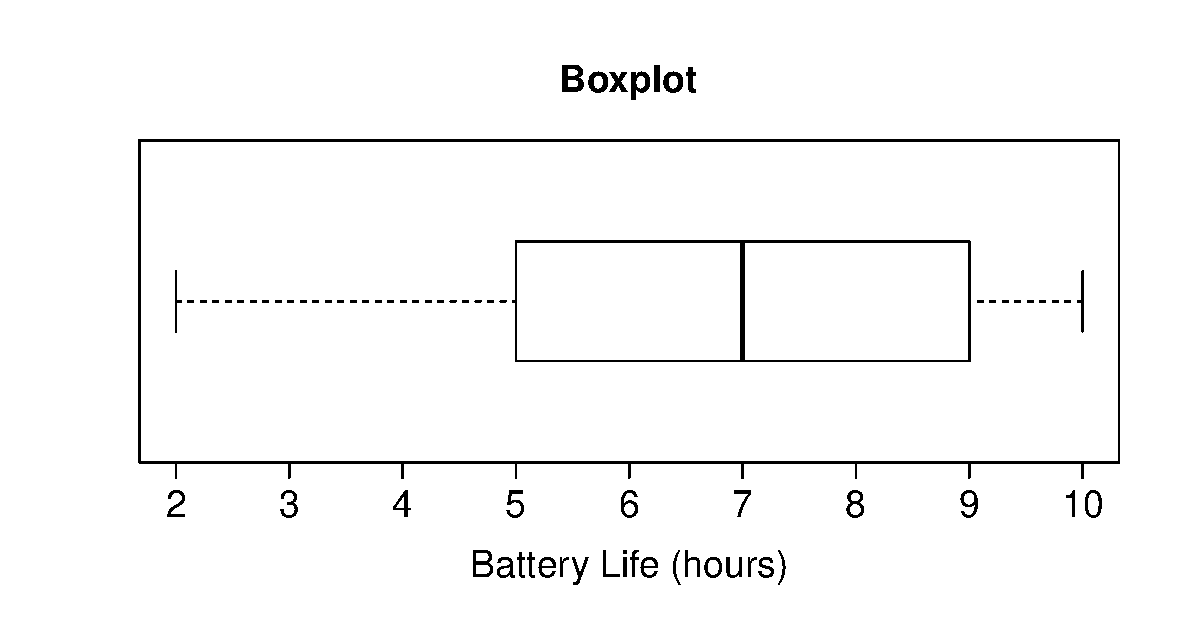
\includegraphics[width=0.8\textwidth, trim = 1.3cm 0.6cm 1cm 0.8cm, clip]{BoxplotB}
\end{center}

{\bf Q5} Based on the above boxplot, what is the value of the $IQR$?\\[0.2cm]
\begin{tabular}{cccc}
{\bf(a)} $8$ hours & {\bf(b)} $2$ hours & {\bf(c)} $4$ hours & {\bf(d)} $9$ hours \\[0.6cm]
\end{tabular}



\rule{\linewidth}{1pt}

\newpage

\section*{Rough Work\\[23cm]}
\section*{\hspace{8cm}$\boxed{\text{Next page: Questions 6 - 10}}$}

\newpage


\section*{Questions 6 - 10}

\rule{\linewidth}{1pt}
\quad\\
Consider the following set of numbers:
\begin{center}
\begin{tabular}{|ccccccccc|}
\hline
&&&&&&&&\\[-0.4cm]
13 & 5 & 21 & 11 & 15 & 13 & 12 & 14 & 8 \\
\hline
\multicolumn{9}{c}{}
\end{tabular}
\end{center}

{\bf Q6} What is the value of the 1st quartile?\\[0.2cm]
\begin{tabular}{cccc}
{\bf(a)} 13 & {\bf(b)} 9.5 & {\bf(c)} 2.5 & {\bf(d)} 14.5 \\[0.6cm]
\end{tabular}


\rule{\linewidth}{1pt}
\begin{center}
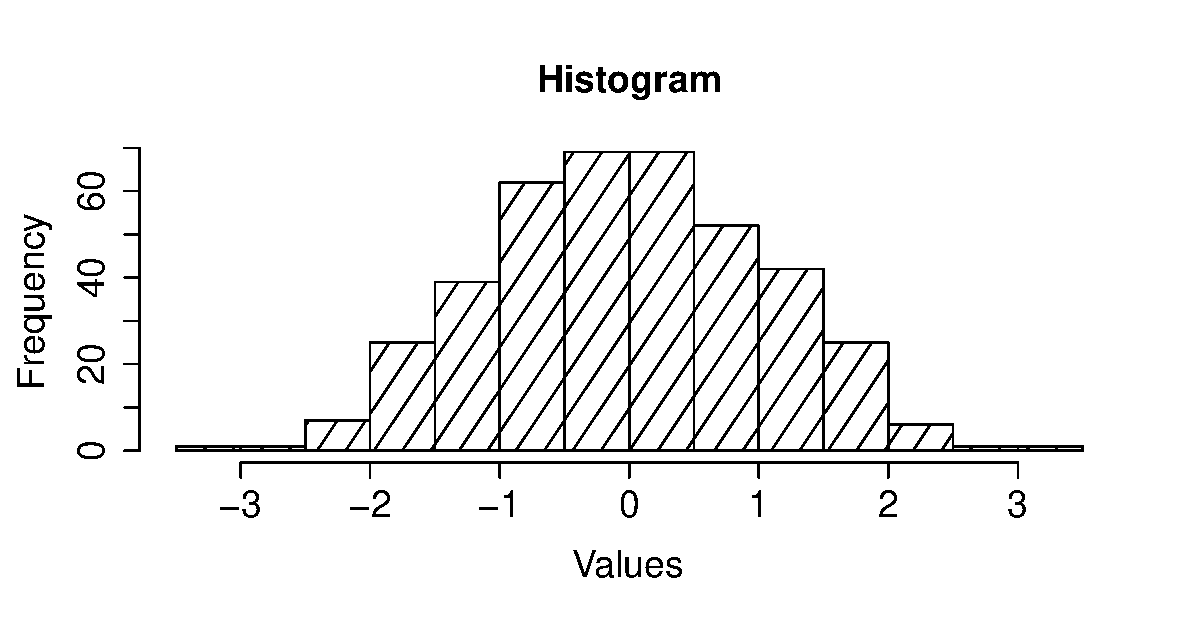
\includegraphics[width=0.8\textwidth, trim = 0.0cm 0.6cm 1.5cm 0.8cm, clip]{Hist}
\end{center}
{\bf Q7} From the above histogram, the distribution of data is:\\[0.2cm]
\begin{tabular}{cccc}
{\bf(a)} frequent & {\bf(b)} right-skewed & {\bf(c)} left-skewed & {\bf(d)} symmetrical \\[0.6cm]
\end{tabular}


\rule{\linewidth}{1pt}
\quad\\
A mobile application developer employs two coders (call them $C_1$ and $C_2$ for simplicity): \mbox{80\% of all code} is written by $C_1$ and the remaining 20\% is written by $C_2$. Given that $C_1$ writes the code, there is 10\% chance that it contains a bug. On the other hand, given that $C_2$ writes the code, there is 30\% chance that it contains a bug.\\{\footnotesize(Note: answers below are given to two decimal places)}\\[0.3cm]

{\bf Q8} Let $B$ represent the event that the code contains a bug. What is the value of $\Pr(B)$?\\[0.2cm]
\begin{tabular}{cccc}
{\bf(a)} 0.03 & {\bf(b)} 0.26 & {\bf(c)} 0.14 & {\bf(d)} 0.40 \\[0.6cm]
\end{tabular}

{\bf Q9} Some code is checked and found to be \emph{bug-free}; what is the probability that $C_2$ wrote it?\\[0.2cm]
%{\footnotesize(answer is given to two decimal places)}\\[0.2cm]
\begin{tabular}{cccc}
{\bf(a)} 0.70 & {\bf(b)} 0.84 & {\bf(c)}  0.16 & {\bf(d)} 0.43 \\[0.6cm]
\end{tabular}


\rule{\linewidth}{1pt}
\quad\\
{\bf Q10} You have 9 t-shirts. You're going on holidays and can only bring 4 of them. How many possible groups of 4 t-shirts are there if one of them is your ``lucky'' t-shirt and you \emph{must} bring it?\\[0.2cm]
\begin{tabular}{cccc}
{\bf(a)} 336 & {\bf(b)} 56 & {\bf(c)} 84 & {\bf(d)} 126  \\[0.6cm]
\end{tabular}

\rule{\linewidth}{1pt}

\newpage

\section*{Rough Work\\[23cm]}
\section*{\hspace{8cm}$\boxed{\text{Next page: Questions 11 - 15}}$}

\newpage

\section*{Questions 11 - 15}


\rule{\linewidth}{1pt}
\quad\\
{\bf Q11} Let $\Pr(A) = 0.6$, $\Pr(B) = 0.7$ and $\Pr(A \cap B) = 0.55$. What is the value of $\Pr(A^c \cap B^c)$? \\[0.2cm]
\begin{tabular}{cccc}
{\bf(a)} 0.75 & {\bf(b)} 0.25  & {\bf(c)} 0.45  & {\bf(d)} 0.42 \\[0.6cm]
\end{tabular}



\rule{\linewidth}{1pt}
\quad\\
Consider the following \emph{joint} distribution for $X$ and $Y$:
\begin{center}
\begin{tabular}{c|c|ccc|c|}
\multicolumn{2}{c}{} & \multicolumn{3}{c}{$X$} & \multicolumn{1}{c}{}\\
\cline{2-6}
&&&&&\\[-0.4cm]
&&                          1 & 2 & 3 & $p(y)$\\
\cline{2-6}
&&&&&\\[-0.3cm]
\multirow{2}{*}{$Y$} & 1 & $0.25$ &  $0.10$  & $0.10$ & $0.45$ \\[0.1cm]
                     & 2 & $0.05$ &  $0.35$  & $0.15$ & $0.55$ \\[0.1cm]
\cline{2-6}
&&&&&\\[-0.3cm]
& $p(x)$ & $0.3$ & $?$ & $0.25$ & 1 \\[0.1cm]
\cline{2-6}
\multicolumn{6}{c}{}\\[-0.4cm]
\end{tabular}
\end{center}
{\footnotesize(Note: answers below are given to two decimal places)}\\[-0.1cm]

{\bf Q12} What is the value of $E(X)$?\\[0.2cm]
\begin{tabular}{cccc}
{\bf(a)} 2.05 & {\bf(b)} 1.95 & {\bf(c)} 1.55 & {\bf(d)} 0.45 \\[0.6cm]
\end{tabular}

{\bf Q13} What is the value of $\Pr(X=3\,|\,Y=1)$?\\[0.2cm]
\begin{tabular}{cccc}
{\bf(a)} 0.22 & {\bf(b)} 0.40 & {\bf(c)} 0.27 & {\bf(d)} 0.11 \\[0.6cm]
\end{tabular}


\rule{\linewidth}{1pt}
\quad\\
There is a 6\% chance of pressing the wrong button on a keyboard and thus make a typographical error. Assuming these errors occur independently, the number of errors in typing $n$ letters is $X \sim$ Binomial$(n,p)$.\\{\footnotesize(Note: answers below are given to four decimal places)}\\[0.3cm]

{\bf Q14} You type 11 letters. What is the probability of making \emph{less than} 2 errors? \\[0.2cm]
%{\footnotesize(hint: cannot use tables)}\\[0.2cm]
\begin{tabular}{cccc}
{\bf(a)} 0.3555 & {\bf(b)} 0.8618 & {\bf(c)} 0.1135 & {\bf(d)} 0.9752 \\[0.6cm]
\end{tabular}

{\bf Q15} You type 100 letters. What is $\Pr(X > 10)$? \\[0.2cm]
%{\footnotesize(hint: use tables)}\\[0.2cm]
\begin{tabular}{cccc}
{\bf(a)} 0.0209 & {\bf(b)} 0.0399 & {\bf(c)} 0.0376 & {\bf(d)} 0.0775 \\[0.6cm]
\end{tabular}

\rule{\linewidth}{1pt}








\newpage

\section*{Rough Work\\[23cm]}
\section*{\hspace{2cm}$\boxed{\text{Don't forget to enter your answers on the last page!}}$}

\newpage


\section*{Useful Formulae: Page 1\\[0.3cm]}
{\bf Histogram:}\\[-0.8cm]
\begin{align*}
\bullet\quad \text{class width} = \frac{\max(x) - \min(x)}{\text{number of classes}}\\
\end{align*}
{\bf Numerical Summaries:}\\[-0.8cm]
\begin{align*}
\bullet\quad \bar x &= \frac{\sum\,x_i}{n}\\[0.6cm]
\bullet\quad s^2 &= \frac{\sum\,x_i^2 - n\,\bar x^2}{n-1}\\[0.6cm]
\bullet\quad \text{Position of } Q_k:& \quad \frac{n+1}{4}\times k \\[0.6cm]
\bullet\quad IQR &= Q_3 - Q_1 \\[0.6cm]
\bullet\quad LF &= Q_1 - 1.5 \times IQR \\[0.6cm]
\bullet\quad UF &= Q_3 + 1.5 \times IQR\\
\end{align*}
{\bf Probability:}\\[-0.8cm]
\begin{align*}
\bullet\quad \Pr(A^c) &= 1 - \Pr(A) \\[1cm]
\bullet\quad \Pr(A \cup B) &= \Pr(A) + \Pr(B) - \Pr(A \cap B)\\[0.6cm]
\bullet\quad \Pr(E_1 \cup E_2 \cup \cdots \cup E_k) &= \Pr(E_1) + \Pr(E_2) + \cdots + \Pr(E_k) \text{\quad{\footnotesize(if mutually exclusive)}}\\[1cm]
\bullet\quad \Pr(A \cap B) &= \Pr(A) \, \Pr(B \, | \, A) = \Pr(B) \, \Pr(A \, | \, B) \\[0.6cm]
\bullet\quad \Pr(E_1 \cap E_2 \cap \cdots \cap E_k) &= \Pr(E_1) \, \Pr(E_2) \, \cdots \, \Pr(E_k) \text{\quad{\footnotesize(if independent)}}\\[1cm]
\bullet\quad \Pr(A\,|\,B) &= \frac{\Pr(A \cap B)}{\Pr(B)} = \frac{\Pr(A) \,\Pr(B\,|\,A)}{\Pr(B)}\\[1cm]
\bullet\quad \text{If $E_1,\ldots, E_k$} & \,\, \text{are mutually exclusive \& exhaustive}\\[0.1cm]
\Rightarrow \Pr(B) &= \Pr(B \cap E_1) + \Pr(B \cap E_2) + \cdots + \Pr(B \cap E_k) \\[0.2cm]
&= \Pr(E_1) \, \Pr(B\,|\,E_1) + \Pr(E_2) \, \Pr(B\,|\,E_2) + \cdots + \Pr(E_k) \, \Pr(B\,|\,E_k)\\
\end{align*}

\newpage

\section*{Useful Formulae: Page 2\\[0.3cm]}
{\bf Counting Techniques:}\\[-0.8cm]
\begin{align*}
\bullet\quad n\,! &= n\times(n-1)\times(n-2)\times\cdots\times3\times2\times 1\\[0.6cm]
\bullet\quad \binom{n}{k} &= \frac{n\,!}{k\,! (n-k)\,!}\\
\end{align*}
{\bf Random Variables:}\\[-0.8cm]
\begin{align*}
\bullet\quad E(X) &= \sum x_i \,\, p(x_i)\\[0.6cm]
\bullet\quad E(X^2) &= \sum x_i^2 \,\, p(x_i)\\[0.6cm]
\bullet\quad Var(X) &= E(X^2) - [E(X)]^2\\[0.6cm]
\bullet\quad Sd(X) &= \sqrt{Var(X)}\\
\end{align*}
{\bf Binomial Distribution:}\\[-0.8cm]
\begin{align*}
\bullet\quad X &\sim \text{Binomial}(n,p)\\[0.6cm]
\bullet\quad \Pr(X=x) &= \binom{n}{x}\,p^x\,(1-p)^{n-x}\\[0.6cm]
\bullet\quad x &\in \{0,1,2,\ldots,n\}\\[0.6cm]
\bullet\quad E(X) &= n\,p \\[0.6cm]
\bullet\quad Var(X) &= n\,p\,(1-p)\\
\end{align*}

\newpage


\begin{adjustwidth}{-1cm}{0cm}
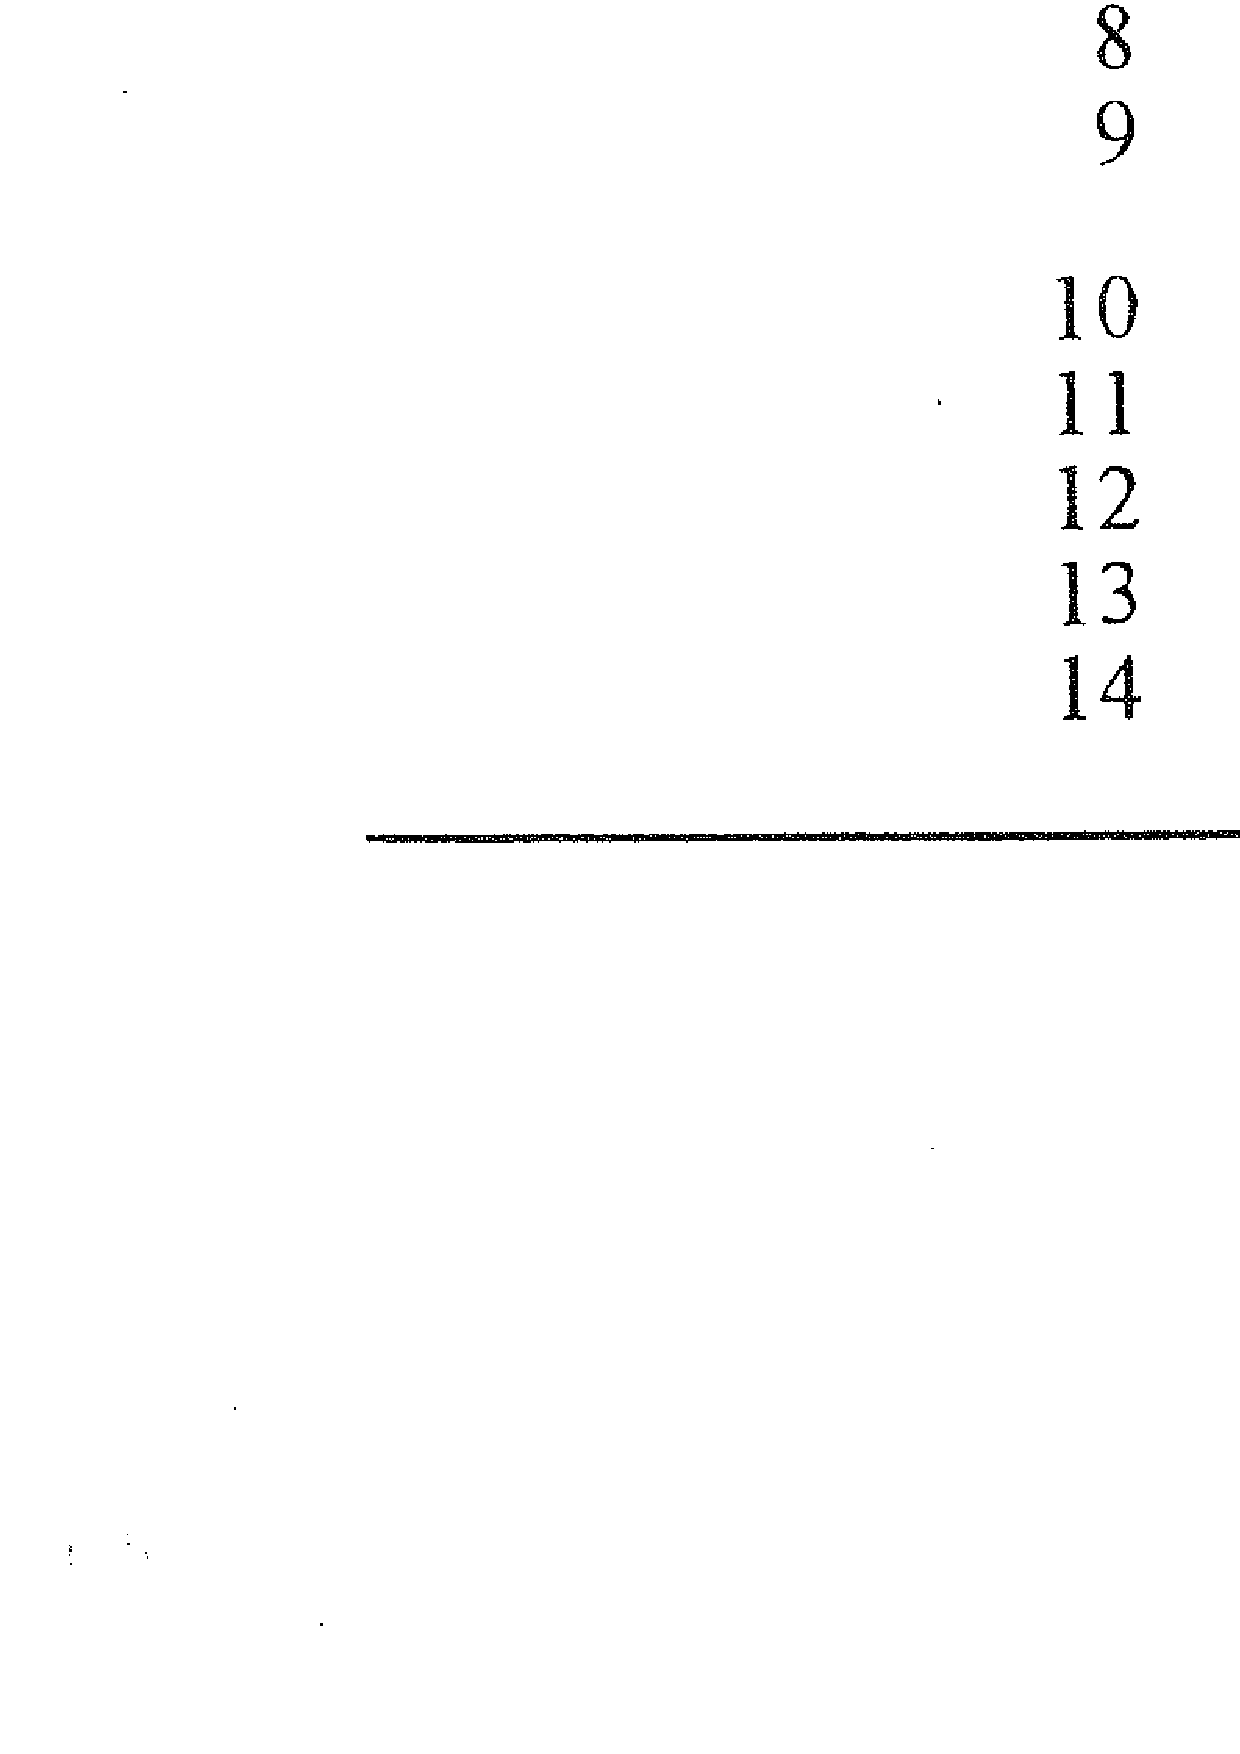
\includegraphics[width=1.1\textwidth, trim = 2cm 4cm 2cm 3cm, clip]{Md1}
\end{adjustwidth}

\newpage

\begin{adjustwidth}{-1cm}{0cm}
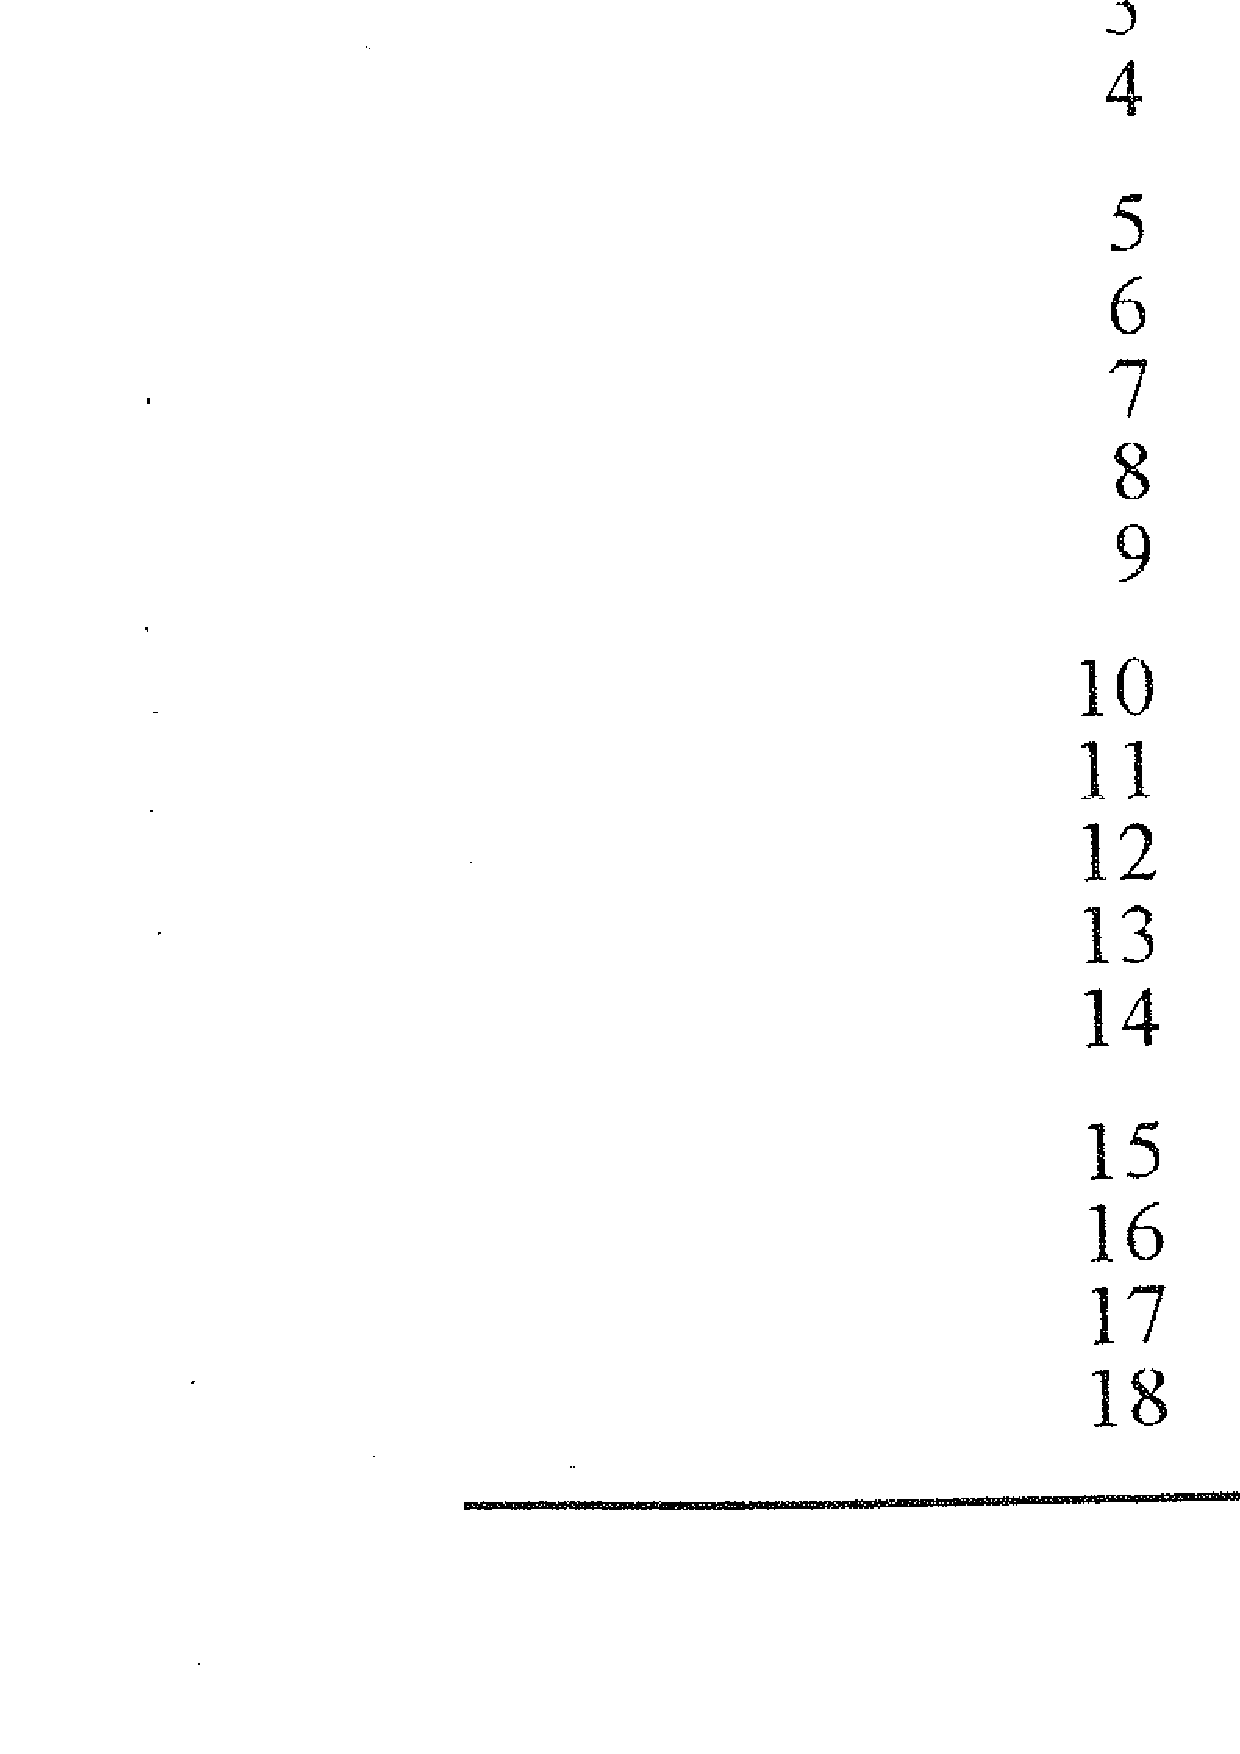
\includegraphics[width=1.1\textwidth, trim = 2cm 4cm 2cm 3cm, clip]{Md2}
\end{adjustwidth}

\newpage

\section*{Answer Sheet\\[0.3cm]}

\subsection*{Name:\quad\underline{\hspace{11.45cm}}\\[0.3cm]}
\subsection*{ID Number:\quad\underline{\hspace{10cm}}\\[0.5cm]}

Enter your answers with an ``X' in the table below.\\[0.3cm]
Do not enter the ``X'' until you have made your \emph{final decision} to avoid scribbling out.\\[0.3cm]
\begin{large}
\begin{center}
\begin{tabular}{|c|c|c|c|c|}
\hline
&&&&\\[-0.4cm]
 & A & B & C & D \\
\hline
&&&&\\[-0.4cm]
Q1 &&&& \\
\hline
&&&&\\[-0.4cm]
Q2 &&&& \\
\hline
&&&&\\[-0.4cm]
Q3 &&&& \\
\hline
&&&&\\[-0.4cm]
Q4 &&&& \\
\hline
&&&&\\[-0.4cm]
Q5 &&&& \\
\hline
\multicolumn{5}{c}{}\\[-0.3cm]
\hline
&&&&\\[-0.4cm]
Q6 &&&& \\
\hline
&&&&\\[-0.4cm]
Q7 &&&& \\
\hline
&&&&\\[-0.4cm]
Q8 &&&& \\
\hline
&&&&\\[-0.4cm]
Q9 &&&& \\
\hline
&&&&\\[-0.4cm]
Q10 &&&& \\
\hline
\multicolumn{5}{c}{}\\[-0.3cm]
\hline
&&&&\\[-0.4cm]
Q11 &&&& \\
\hline
&&&&\\[-0.4cm]
Q12 &&&& \\
\hline
&&&&\\[-0.4cm]
Q13 &&&& \\
\hline
&&&&\\[-0.4cm]
Q14 &&&& \\
\hline
&&&&\\[-0.4cm]
Q15 &&&& \\
\hline
\end{tabular}
\end{center}
\end{large}


\end{document} 